
\documentclass[]{report}

\voffset=-1.5cm
\oddsidemargin=0.0cm
\textwidth = 480pt

\usepackage{framed}
\usepackage{subfiles}
\usepackage{graphics}
\usepackage{newlfont}
\usepackage{eurosym}
\usepackage{amsmath,amsthm,amsfonts}
\usepackage{amsmath}
\usepackage{enumerate}
\usepackage{color}
\usepackage{multicol}
\usepackage{amssymb}
\usepackage{multicol}
\usepackage[dvipsnames]{xcolor}
\usepackage{graphicx}
\begin{document}
	
	\section{Network Analysis — Resource Scheduling }	
	%===============%
	
	\subsection*{Objectives} After studying this chapter you will 
	\begin{itemize}
		\item  understand the principles of Resource Scheduling 
		\item  know how to draw a Gantt chart 
		\item  be able to prepare a Resource Aggregation Profile 
		\item  know how to use Resource Levelling 
		\item  be able to prepare a Resource Allocation Profile. 
	\end{itemize}
	\subsection*{Resources and networks} 
	The usefulness of networks is not confined only to the time and cost factors wh been discussed so far. Considerable assistance in planning and controlling the resources can be given to management by appropriate development of the basic techniques. Project resources. The resources (men of varying skills, machines of all ty required materials, finance, and space) used in a project are subject to varying and loadings as the project proceeds. Management need to know what activi what resources are critical to the project duration and if resource limitatic shortage of materials, limited number of skilled craftsmen) might delay the proj€ also wish to ensure, as far as possible, constant work rates to avoid paying ovt one stage of a project and having short time working at another stage. 
	\subsection*{Resource scheduling requirements} To be able to schedule the resource requirements for a project the following d required.
	\begin{enumerate}[(a)]
		\item The customary activity times, descriptions and sequences as previously des 
		\item The resource requirements for each activity showing the classification of the and the quantity required.
		\item The resources in each classification that are available to the project. If var availability are likely during the project life, these must also be specified. 
		\item Any management restrictions that need to be considered e.g. which activiti may not be split or any limitations on labour mobility. 
	\end{enumerate}
	\subsection*{Resources scheduling example, using a Gantt chart} A simple project has the following time and resource data (for simplicity, on resource of labour is considered but similar principles would apply to othe inter-changeable resources). 
	348 
	
	
	%==========%
	
	
	% 25 Network analysis — resource scheduling 
	Project data 
	\begin{tabular}{cccc}
		Activity  & Preceding activity &  Duration (days) & Labour requirements \\ \hline 
		A & — & 1 &  2 men \\ \hline 
		B & — & 2 & 1 man  \\ \hline 
		C & A & 1 & 1 man \\ \hline 
		D &   & 5 & 1 man \\ \hline 
		E & B & 1 & 1 man \\ \hline 
		F & C & 1 & 1 man \\ \hline 
	\end{tabular}
	
	Resource constraint, 2 men only available 
	\begin{figure}[h!]
\centering
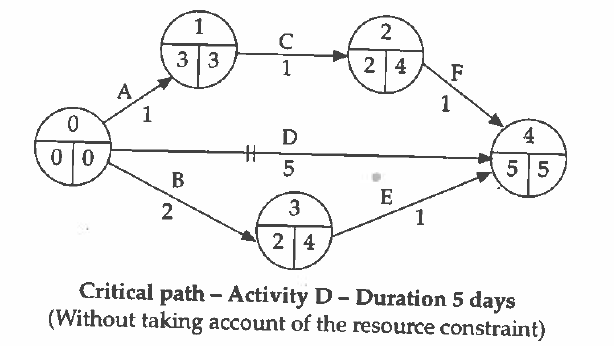
\includegraphics[width=0.4\linewidth]{images4/349-a}
\caption{}
\label{fig:349-a}
\end{figure}

	Critical path — Activity D — Duration 5 days (Without taking account of the resource constraint) Resource Scheduling Steps 
\begin{description}
\item[Step 1] Draw the activity times on a Gantt or Bar Chart based on their ESTs 
	
\begin{figure}[h!]
\centering
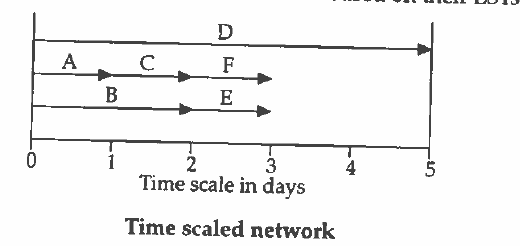
\includegraphics[width=0.4\linewidth]{images4/349-b}
\caption{}
\label{fig:349-b}
\end{figure}

	
	Time scaled network 
\item[Step 2] Based on the time bar chart prepare a Resource Aggregation Profile i.e. total resource requirements in each time period. 
\begin{figure}[h!]
\centering
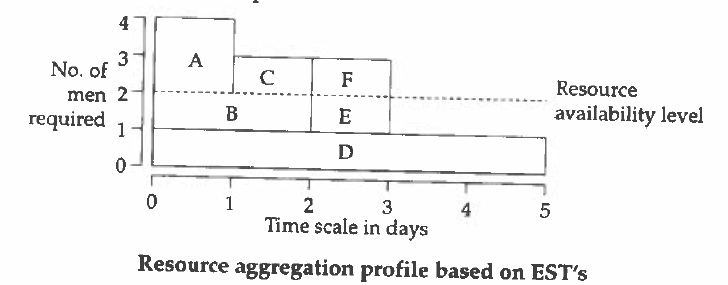
\includegraphics[width=0.4\linewidth]{images4/349-c}
\caption{}
\label{fig:349-c}
\end{figure}
% Time scale in days 
% Resource aggregation profile based on EST's 
\item[Step 3]Examination of the above profile shows that at times more resources are required than are available if activities commence at their EST's. 

	
	%================%
%	25 Network analysis - resource. scheduling 
The ESTs/LSTs on the network show that float is available for activities A, C, F, B and E. 
	
	Having regard to these floats it is necessary to 'smooth out' the resource requirements so that the resources required do not exceed the resource constraint, i.e. delay 
	the commencement of activities (within their float) and if this procedure is still not sufficient then delay the project as a whole. Carrying out this procedure results 
	in the following resource profile. 
	
\begin{figure}[h!]
\centering
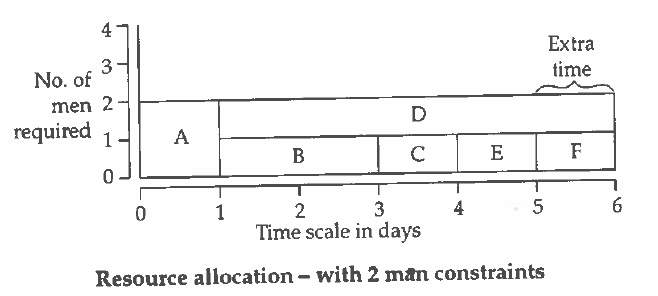
\includegraphics[width=0.4\linewidth]{images4/350-a}
\caption{}
\label{fig:350-a}
\end{figure}

%	Resource allocation - with 2 man constraints 
Note: This procedure is sometimes termed resource levelling. \item[Step 4] Because of the resource constraint of 2 men it has been necessary to extend the project duration by 1 day. Assume that management state that the original project duration (5 days) must not be extended and they require this to be achieved with the minimum extra resources. In such cases a similar process of varying activity start times within their float is carried out, resulting in the following resource profile. 

\begin{figure}[h!]
\centering
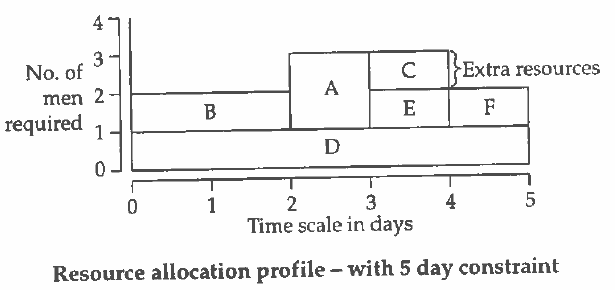
\includegraphics[width=0.4\linewidth]{images4/350-b}
\caption{}
\label{fig:350-b}
\end{figure}
 Resource allocation profile with 5 day constraint 
	\item[Step 5] The above profile shows that to achieve the 5 day duration it is necessary to have 3 men available from day 2 to day 4. 
\end{description}
	\subsection*{Summary}
	\begin{enumerate}[(a)]
		\item To enable resource scheduling to be carried out the resource requirements for each activity must be specified. 
		\item In addition the various resources involved (men, machinery etc) must be classified and the availability and constraints specified. 
		\item After calculating the critical path in the usual manner a Resource Aggregation Profile(s) is prepared i.e. the amount of the resource(s) required in
		each time period of the project based on the EST's of each activity. 
		\item If the resource aggregation indicates that a constraint is being exceeded, and float is available the resource usage is 'smoothed' i.e. the start of activities is delayed. 
	\end{enumerate}
	%============================%
	
	% 25 Network analysis - resource scheduling 
	\subsection*{Points to note} 
The smoothing of resource profiles is largely a matter of experimentation but if the time for the project is fixed concentrate attention on those activities with free float. % (described in Chapter 23). 

\subsection*{Self review questions} 
Numbers in brackets refer to paragraph numbers 
\begin{itemize}
	\item What data are required to be able to carry out resource scheduling on a network? 
	\item  What is a resource aggregation profile? 
	\item  What is resource levelling? 
\end{itemize}

	\subsection*{Exercises with answers}
\begin{enumerate}
	\item A project has the following activity durations and resource requirements. 

\begin{center}
\begin{tabular}{|c|c|c|c|}
Activity & Preceding  & Duration & Resource \\
& activity & & requirements \\
&	(days)&& (units) \\ \hline
	A & — & 6 & 3  \\ \hline
	B & — & 3 & 2  \\ \hline
	C & — & 2 & 2  \\ \hline
	D & C & 2 & 1 \\ \hline
	E & B & 1 & 2 \\ \hline
	F & D & 1 & 1 \\ \hline
\end{tabular}
\end{center}	
	Assuming no restrictions show the network, critical path and resource requirements on a 
	day by day basis, assuming that starts are made on the EST of each activity. 
\item Assume that there are only 6 units of resources what would be the plan? 
\end{enumerate}
\newpage	
	\subsection*{Answers to exercises}

\begin{enumerate}
	\item Exercise 1

	\begin{figure}[h!]
\centering
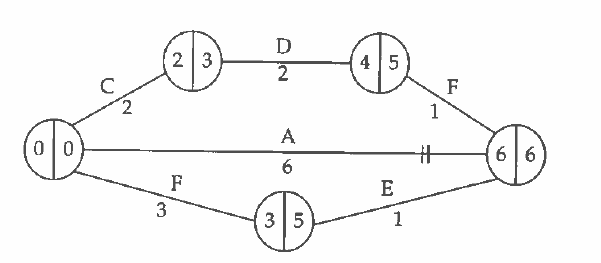
\includegraphics[width=0.4\linewidth]{images4/351-a}
\caption{}
\label{fig:351-a}
\end{figure}
\begin{figure}[h!]
\centering
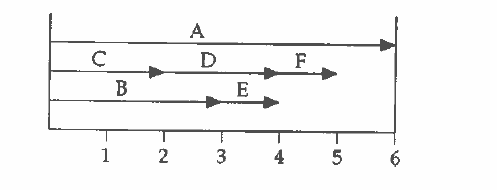
\includegraphics[width=0.4\linewidth]{images4/351-b}
\caption{}
\label{fig:351-b}
\end{figure}

	%===================================%
	% Page 352
\begin{figure}[h!]
\centering
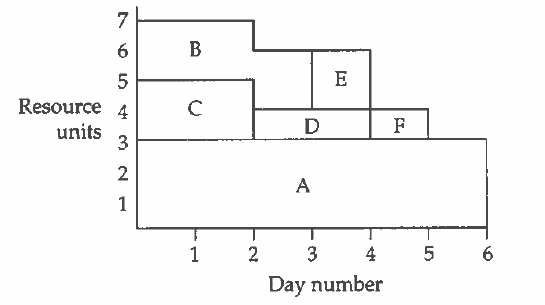
\includegraphics[width=0.4\linewidth]{images4/352-a}
\caption{}
\label{fig:352-a}
\end{figure}
\item Exercise 2:  Delay start of B/E until day 2 resulting in 
\begin{figure}[h!]
\centering
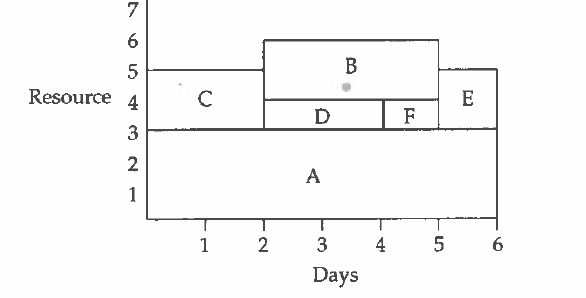
\includegraphics[width=0.4\linewidth]{images4/352-b}
\caption{}
\label{fig:352-b}
\end{figure}
\end{enumerate}
	
	
	
\end{document}